\chapter{Detekcja obiektów}
\section{Opis procesu uczenia}
\label{opis}

\hspace{0.5cm}
Model został stworzony i uczony na platformie Google Collaboratory z wykorzystaniem procesora graficznego Nvidia Tesla T4 oferowanego przez środowisko. Przy każdym uruchomieniu programu uczącego dobierane zostały osobno parametry tj.
\begin{itemize}
    \item[--] architektura (ResNet50, ResNet101, ResNet152 lub VGG19),
    \item[--] ilość epok,
    \item[--] zdjęcia zbioru uczącego i walidacyjnego,
    \item[--] ilość zdjęć przekazywanych do przetworzenia jednocześnie,
    \item[--] ilość kroków w jednej epoce,
    \item[--] współczynnik szybkości uczenia.
\end{itemize}

\hspace{0.5cm}
Ze względu na długi czas uczenia, większość modeli tworzona była w kilku częściach. Po ukończeniu ewaluacji każdej kolejnej epoki tworzony był możliwy do wykorzystania model a~po zakończeniu całego procesu wykreślone zostały wykresy zawierające podstawowe informacje (przykładowe wyniki na rysunku \ref{fig:inf}) np. wykres straty zbioru uczącego (pomarańczowy) i~walidacyjnego (niebieski) na przestrzeni wszystkich epok.

\begin{figure}[H]
\hspace{-1.5cm}
\subfloat[Wykres straty treningu i straty \\ walidacji.]{\label{inf1}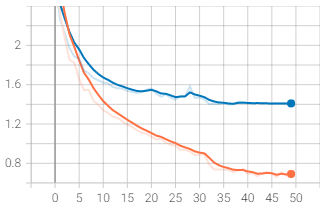
\includegraphics[width=.4\linewidth]{Obrazy/Rozdzial05/info/strata.png}}
\subfloat[Wykres wartości współczynnika szybkości uczenia.]{\label{inf2}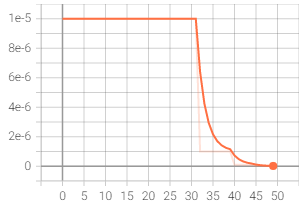
\includegraphics[width=.4\linewidth]{Obrazy/Rozdzial05/info/lr.png}}
\subfloat[Wykres parametru AP.]{\label{inf3}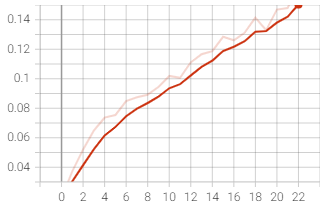
\includegraphics[width=.4\linewidth]{Obrazy/Rozdzial05/info/precyzja.png}}
\caption{Zestawienie graficznego przedstawienia informacji istotnych przy ewaluacji każdego modelu na przestrzeni epok.}
\label{fig:inf}
\end{figure}

\hspace{0.5cm}
W przypadku, gdy przez dwie epoki sieć nie poczyniła żadnych postępów w swoim treningu, szybkość uczenia zostanie automatycznie zmniejszona. Wynika to ze sposobu implementacji  wykorzystywanego repozytorium.

\begin{figure}[H]
\centering
\subfloat[Stała wartość parametru w trakcie całego procesu.]{\label{lr1}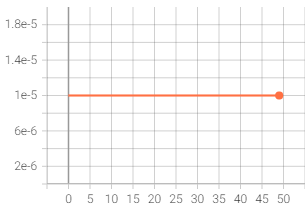
\includegraphics[width=.4\linewidth]{Obrazy/Rozdzial05/info/lr2.png}}
\hspace{0.5cm}
\subfloat[Automatycznie dostosowana wartość parametru.]{\label{lr2}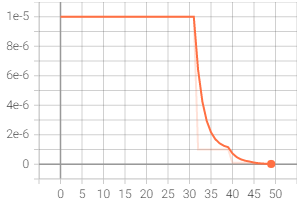
\includegraphics[width=.4\linewidth]{Obrazy/Rozdzial05/info/lr3.png}}\hfill
\caption{Porównanie wykresów wartości parametru szybkości uczenia na przestrzeni 80 epok.}
\label{fig:lr_auto}
\end{figure}

\hspace{0.5cm}
Na koniec została wykonana próba zastosowania modelu w praktyce. W połączeniu z~wartościami liczbowymi generowanymi przez model poddano subiektywnej ocenie na podstawie otrzymanych wyników (rys. \ref{fig:graf}). 

\begin{figure}[H]
    \centering
    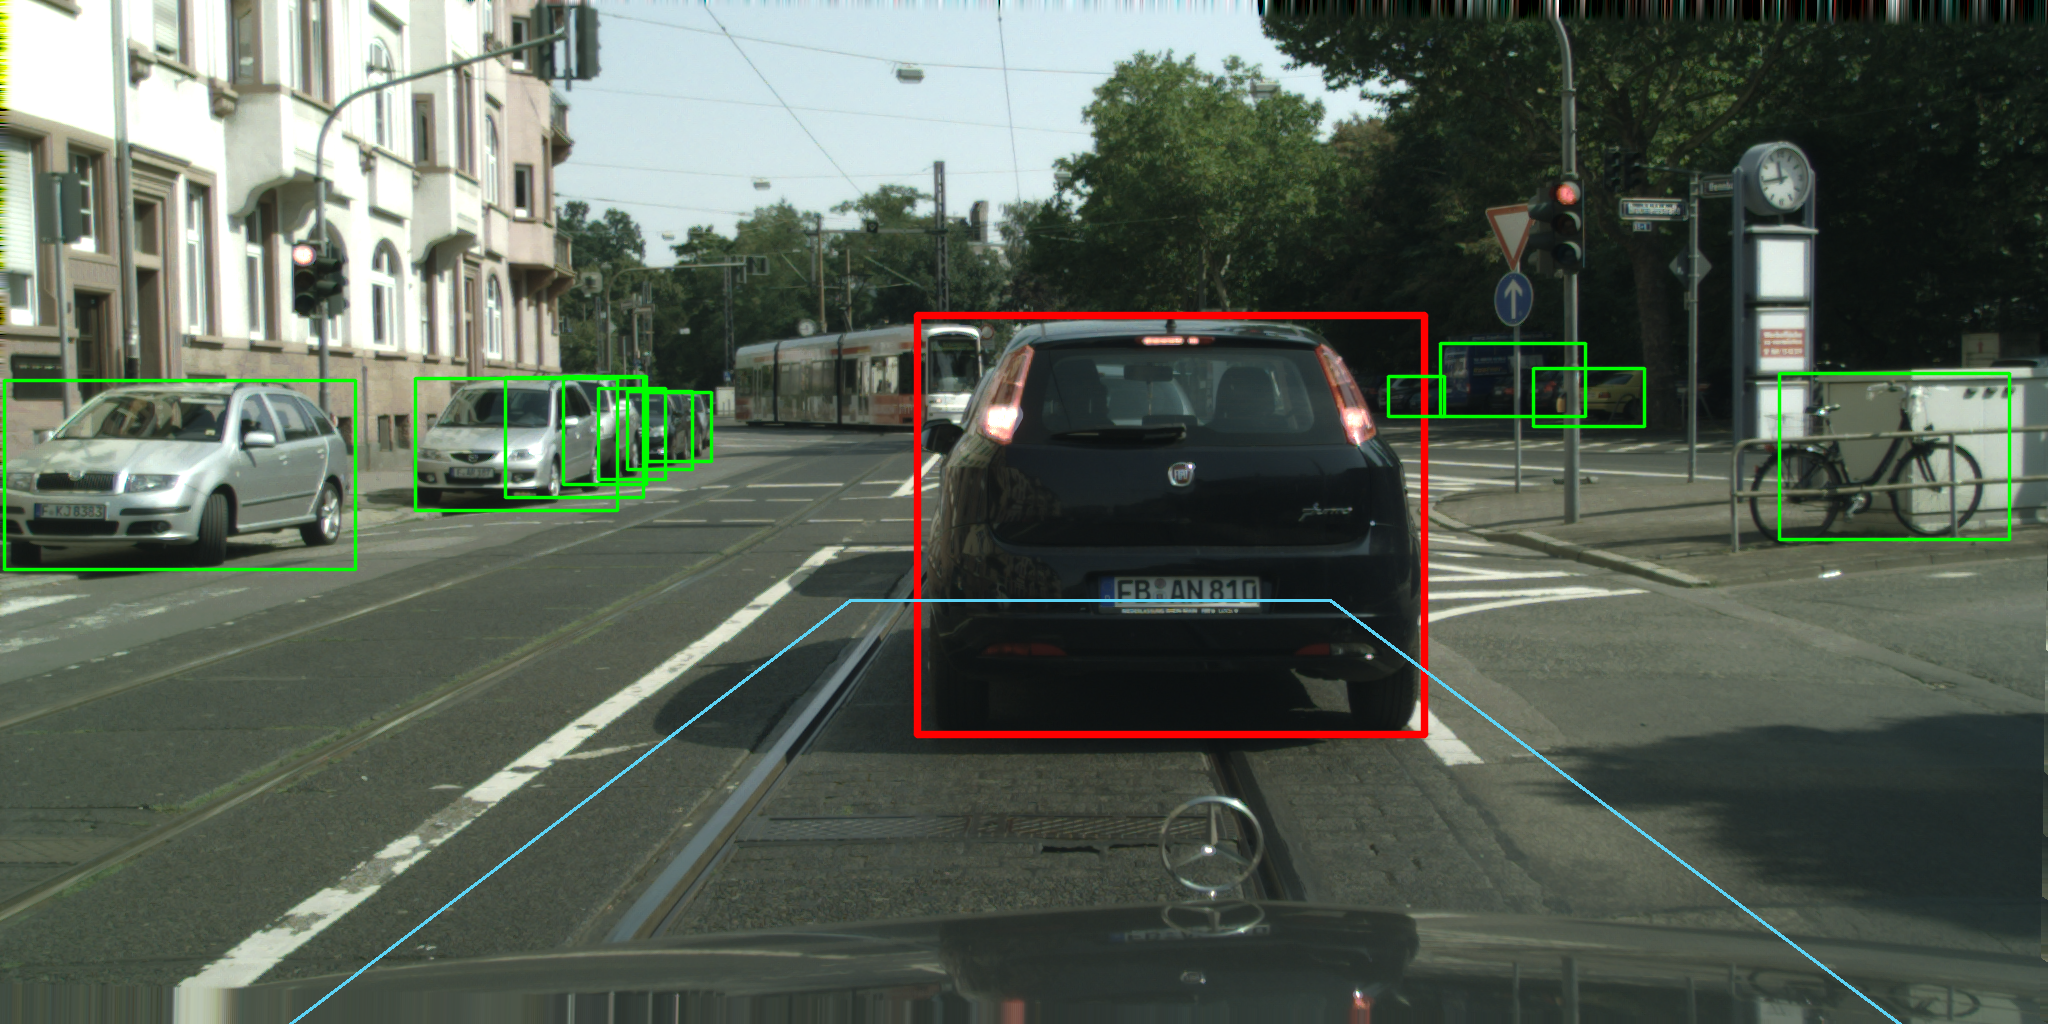
\includegraphics[width=0.7\linewidth]{Obrazy/Rozdzial05/info/przyklad.png}
    \caption{Przykładowa detekcja obiektów na zdjęciu.}
    \label{fig:graf}
\end{figure}

\hspace{0.5cm}
Trening każdej z sieci zakończono po osiągnięciu określonej liczby epok, bez względu na otrzymane rezultaty.

\section{Porównanie wyników}

\hspace{0.5cm}
Ewaluacja wyników odbywała się w kilku etapach, w~zależności od parametru, który był w~danym momencie zmieniany przed rozpoczęciem uczenia. W celu określenia jakości każdego z otrzymanych końcowych modeli dla każdej zastosowanej architektury wykorzystane zostały wykresy strat treningu i walidacji, wykresy parametru szybkości uczenia, metryki AP oraz subiektywna ocena jakościowa.

\hspace{0.5cm}
Metryka AP określa stosunek poprawnych detekcji do sumy poprawnych detekcji (poprawnym wyznaczeniu lokalizacji i klasyfikacji) oraz fałszywych detekcji obiektów. Wysoka wartość współczynnika AP świadczy o tym, że otrzymany system nie generuje wielu fałszywych predykcji. Metryka dzielona jest na kategorie
\begin{itemize}
    \item[--] AP - uśredniona precyzja dla każdej wartości IoU pochodzącego z przedziału 0.5-0.95 (przykładowy wykres opisujący tą wartość przedstawiony na rysunku \ref{inf3}),
    \item[--] AP50 - procent ramek, dla których stosunek IoU wynosi przynajmniej 50\%,
    \item[--] AP75 - procent ramek, dla których stosunek IoU wynosi przynajmniej 75\%.
\end{itemize}

\hspace{0.5cm}
Wartość IoU jest miarą dokładności określenia położenia oraz rozmiaru obiektu. Miara obliczana jest na podstawie rzeczywistej ramki obiektu oraz ramki zwracanej przez sieć neuronową. Zdefiniowana jest jako stosunek iloczynu (część wspólna) ramek do ich sumy.


% Na podstawie wyników zawartych w tablicy 2
% zaobserwować można, że wyższe wyniki osiągane są dla
% mniejszych wartości IoU, co oznacza że dopasowanie ramek
% do wymiarów obiektów nie jest idealne. System uzyskał
% gorsze wyniki dla małych obiektów, co było spodziewanym
% rezultatem. Jest to cecha sieci YOLO, której szybsze
% działanie uzyskane jest kosztem gorszej detekcji małych
% obiektów [



% \hspace{0.5cm}
% Do porównania wyników wykorzystano uśrednioną metrykę AP dla wszystkich rodzajów zdjęć.

% \begin{table}[H]
%     \centering
%     \caption{Porównanie metryk dla ramek.}
%     \begin{center}
%         \begin{tabular}{|l|l|l|l|c|c|c|c|}
%         \hline
%         \multicolumn{3}{|c|}{Hiperparametry}&\multicolumn{1}{|c|}{IoU}&ResNet50&ResNet101&Resne152&VGG19\\ \hline
%         \multirow{18}{*}{\parbox{2cm}{epoch = 50 steps = 400}}&\multirow{9}{*}{b = 1}&\multirow{3}{*}{lr=-3}&0.5:0.95&0.000&0.000&0.000&0.004\\ \cline{4-8}
%                                                                                                             &&&0.5&0.000&0.000&0.000&0.016\\ \cline{4-8}
%                                                                                                             &&&0.75&0.000&0.000&0.000&0.001\\ \cline{3-8}
                                                                                                            
%                                                                                     &&\multirow{3}{*}{lr=-5}&0.5:0.95&0.155&0.168&0.184&0.122\\ \cline{4-8}
%                                                                                                             &&&0.5&0.302&0.321&0.350&0.242\\ \cline{4-8}
%                                                                                                             &&&0.75&0.138&0.153&0.172&0.105\\ \cline{3-8}
                                                                                                            
%                                                                                     &&\multirow{3}{*}{lr=-7}&0.5:0.95&0.014&0.016&0.017&0.007\\ \cline{4-8}
%                                                                                                             &&&0.5&0.045&0.049&0.052&0.023\\ \cline{4-8}
%                                                                                                             &&&0.75&0.005&0.006&0.005&0.001\\ \cline{2-8}
                                                                                                            
%                                                                 &\multirow{9}{*}{b = 3}&\multirow{3}{*}{lr=-3}&0.5:0.95&0.101&0.000&0.000&0.122\\ \cline{4-8}
%                                                                                                             &&&0.5&0.195&0.000&0.000&0.230\\ \cline{4-8}
%                                                                                                             &&&0.75&0.092&0.000&0.000&0.113\\ \cline{3-8}
                                                                                                            
%                                                                                     &&\multirow{3}{*}{lr=-5}&0.5:0.95&0.166&0.188&0.000&0.170\\ \cline{4-8}
%                                                                                                             &&&0.5&0.341&0.364&0.000&0.327\\ \cline{4-8}
%                                                                                                             &&&0.75&0.141&0.176&0.000&0.157\\ \cline{3-8}
                                                                                                            
%                                                                                     &&\multirow{3}{*}{lr=-7}&0.5:0.95&0.022&0.023&0.026&0.015\\ \cline{4-8}
%                                                                                                             &&&0.5&0.061&0.065&0.072&0.043\\ \cline{4-8}
%                                                                                                             &&&0.75&0.012&0.010&0.013&0.006\\ \hline             
%         \end{tabular}
%     \end{center}
%     \label{tab:AP}
% \end{table}

% \begin{table}[H]
%     \centering
%     \begin{center}
%         \begin{tabular}{|l|l|l|l|c|c|c|c|}
%         \hline
%         \multicolumn{3}{|c|}{Hiperparametry}&\multicolumn{5}{|c|}{Architektury sieci}\\ \hline
%         \parbox[t]{2mm}{\multirow{19}{*}{\rotatebox[origin=c]{90}{epoch = 50 \ \ \ steps = 400}}}&\parbox{1.5cm}{Batch size}&\parbox{2cm}{Learning rate}&IoU&ResNet50&ResNet101&ResNet152&VGG19\\ \cline{2-8}
%         %\multirow{18}{*}{\parbox{2cm}{epoch = 50 steps = 400}}&\multirow{9}{*}{b = 1}&\multirow{3}{*}{lr=-3}&0.5:0.95&r1&r2&r3&v\\ \cline{4-8}
%         &\multirow{9}{*}{1}&\multirow{3}{*}{-3}&0.5:0.95&r1&r2&r3&v\\ \cline{4-8}
%                                                                                              &&&0.5&r1&r2&r3&v\\ \cline{4-8}
%                                                                                              &&&0.75&r1&r2&r3&v\\ \cline{3-8}
%                                                                      &&\multirow{3}{*}{-5}&0.5:0.95&r1&r2&r3&v\\ \cline{4-8}
%                                                                                              &&&0.5&r1&r2&r3&v\\ \cline{4-8}
%                                                                                              &&&0.75&r1&r2&r3&v\\ \cline{3-8}
%                                                                      &&\multirow{3}{*}{-7}&0.5:0.95&r1&r2&r3&v\\ \cline{4-8}
%                                                                                              &&&0.5&r1&r2&r3&v\\ \cline{4-8}
%                                                                                              &&&0.75&r1&r2&r3&v\\ \cline{2-8}
%                                                 &\multirow{9}{*}{3}&\multirow{3}{*}{-3}&0.5:0.95&r1&r2&r3&v\\ \cline{4-8}
%                                                                                              &&&0.5&r1&r2&r3&v\\ \cline{4-8}
%                                                                                              &&&0.75&r1&r2&r3&v\\ \cline{3-8}
%                                                                      &&\multirow{3}{*}{-5}&0.5:0.95&r1&r2&r3&v\\ \cline{4-8}
%                                                                                              &&&0.5&r1&r2&r3&v\\ \cline{4-8}
%                                                                                              &&&0.75&r1&r2&r3&v\\ \cline{3-8}
%                                                                      &&\multirow{3}{*}{-7}&0.5:0.95&r1&r2&r3&v\\ \cline{4-8}
%                                                                                              &&&0.5&r1&r2&r3&v\\ \cline{4-8}
%                                                                                              &&&0.75&r1&r2&r3&v\\ \hline                                                                                          
%         \end{tabular}
%     \end{center}
%     \label{tab:multicol}
% \end{table}

\subsection{Wpływ ilości epok}
% Podczas uczenia sieci neuronowej trzeba wykonać bardzo wiele kroków algorytmu uczenia zanim błąd stanie się akceptowalnie mały. Tymczasem zbiór uczący zawiera zwykle ograniczoną liczbę przypadków uczących, w typowych przypadkach setki lub nawet tysiące razy
% mniej liczną niż liczba koniecznych kroków algorytmu uczenia. Z tego zestawienia wynika, że
% zbiór uczący musi być wykorzystywany w procesie uczenia wielokrotnie. Dla zaznaczenia
% tego faktu wprowadzono pojęcie epoki, rozumiejąc pod tym pojęciem jednorazowe użycie
% w procesie uczenia wszystkich przypadków uczących zawartych w zbiorze uczącym. Po
% wykonaniu wszystkich kroków należących do jednej epoki algorytm uczący dokonuje oceny
% zdolności sieci do generalizacji wyników uczenia przy wykorzystaniu zbioru walidacyjnego. Po stwierdzeniu, że zarówno błąd obliczany na zbiorze uczącym, jak i błąd wyznaczony
% dla zbioru walidacyjnego nadal jeszcze obiecująco maleją – algorytm uczący wykonuje
% następną epokę. W przeciwnym przypadku proces uczenia zostaje zatrzymany.

\hspace{0.5cm}
Epoka jest rozumiana jako jednorazowe użycie wszystkich przypadków uczących tj. zdjęć z~adnotacjami, zawartych w zbiorze uczącym w procesie uczenia sieci. Po każdej z nich wykonywana została ewaluacja z wykorzystaniem zbioru walidacyjnego tak jak zostało to wspomniane w punkcie \ref{opis}. Jeżeli strata zarówno dla zbioru uczącego jak i walidacyjnego nadal maleje, algorytm uczący wykona następną epokę. W innym przypadku proces uczenia powinien się zakończyć lub w zależności od wykorzystywanego programu powinien odpowiednio dostosować parametry (np. szybkość uczenia) w celu poszukiwania mniejszego wyniku \cite{Leksykon}.


\hspace{0.5cm}
Na rysunku \ref{fig:epoka} przedstawiony został wykres straty zbioru uczącego i~walidacyjnego z zaznaczonymi trzema różnymi momentami uczenia sieci, gdy jedynym parametrem poddawanym zmianie była ilość epok uczenia.

\begin{figure}[H]
    \centering
    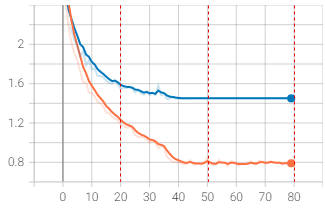
\includegraphics[width=0.5\linewidth]{Obrazy/Rozdzial05/epoka/zamieniony.png}
    \caption{Wykres straty zbioru treningowego i walidacyjnego dla modelu ResNet50 z zaznaczonymi trzema różnymi etapami pobierania modeli.}
    \label{fig:epoka}
\end{figure}

\hspace{0.5cm}
Każdy z tych przypadków wykorzystano do detekcji obiektów na wybranym obrazie i~zestawiono dla porównania na rysunku \ref{fig:epokaporownanie}.

\begin{figure}[H]
    \hspace{2.4cm}
        \subfloat[Liczba epok równa 20.]{\label{e20}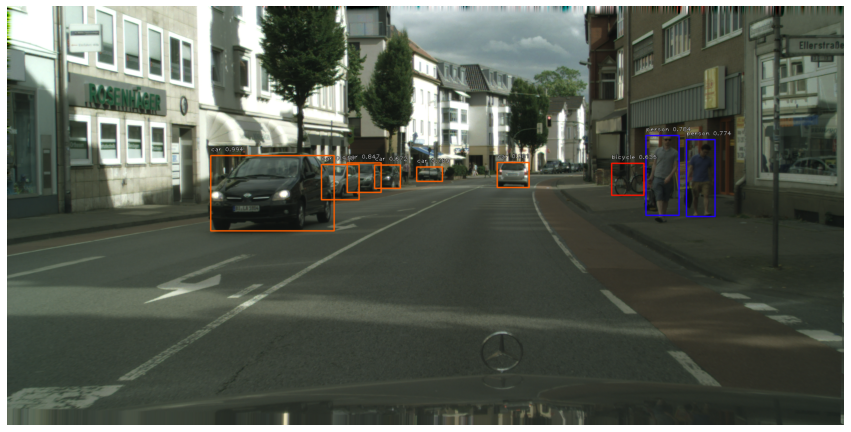
\includegraphics[width=.7\linewidth]{Obrazy/Rozdzial05/epoka/e20.png}}\hfill
    \end{figure}
    \begin{figure}[H]\ContinuedFloat
    \centering
        \subfloat[Liczba epok równa 50.]{\label{e50}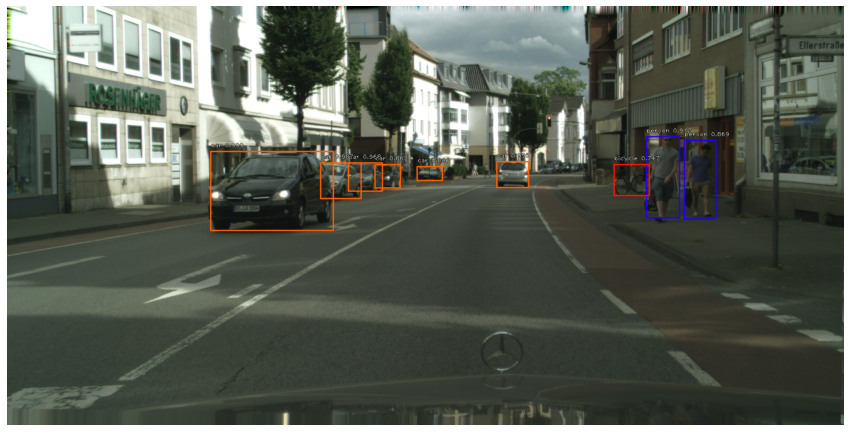
\includegraphics[width=.7\linewidth]{Obrazy/Rozdzial05/epoka/e50.png}}\hfill
        \subfloat[Liczba epok równa 80.]{\label{e80}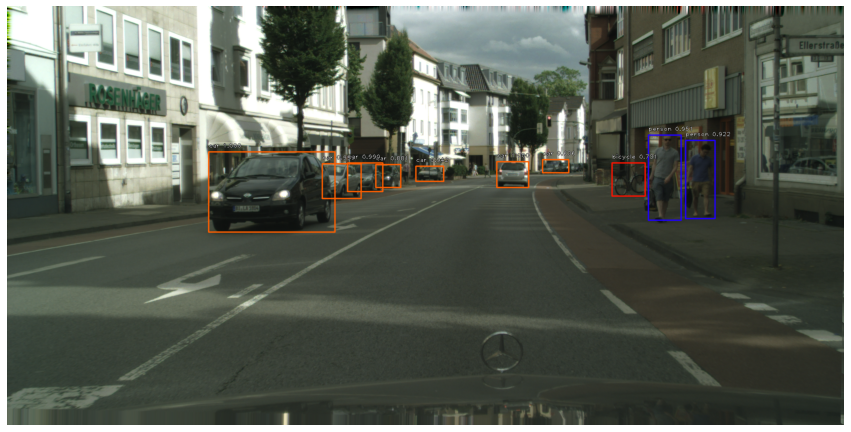
\includegraphics[width=.7\linewidth]{Obrazy/Rozdzial05/epoka/e80.png}}\hfill
    \caption{Porównanie wykresów strat i walidacji dla przykładowej architektury (ResNet50) i różnej ilości epok.}
    \label{fig:epokaporownanie}
\end{figure}

\hspace{0.5cm}
Wygenerowane wykresy strat jak i ocena wizualna oraz wynik prawdopodobieństwa obiektu pozwalały określić, czy ilość epok pozwoliła otrzymać wystarczający model sieci, czy wymagał kontynuacji treningu.

\begin{table}[H]
    \centering
    \caption{Porównanie wartości pewności z jaką sieć określa odnalezione obiekty.}
    \begin{tabular}{|c||c|c|c|}
    \hline
    \multirow{2}{*}{Obiekt}&\multicolumn{3}{|c|}{Epoka} \\ \cline{2-4}
    &20&50&80 \\ \hline
    \multirow{2}{*}{Człowiek} & 0.784 & 0.949 & 0.951 \\ \cline{2-4}
    & 0.774 & 0.569 & 0.922 \\ \hline
    \multirow{7}{*}{Samochód} & 0.944 & 0.999 & 1 \\ \cline{2-4}
    & 0.959 & 0.986 & 0.999 \\ \cline{2-4}
    & 0.847 & 0.968 & 0.999 \\ \cline{2-4}
    & 0.672 & 0.963 & 0.994 \\ \cline{2-4}
    & 0.689 & 0.946 & 0.948 \\ \cline{2-4}    
    & 0.857 & 0.955 & 0.980 \\ \cline{2-4}
    & --- & --- & 0.986 \\ \hline
    Rower & 0.635 & 0.747 & 0.781 \\
    \hline
    \end{tabular}
    \label{tab:prawdopodobienstwo}
\end{table}

\hspace{0.5cm}
Ostatecznie biorąc pod uwagę wyniki z tabeli \ref{tab:prawdopodobienstwo} oraz zdjęcia z rysunku \ref{fig:epokaporownanie} widoczne jest, że na wszystkich przedstawionych etapach sieć była w stanie zwrócić wystarczające wyniki detekcji, mimo że zgodnie z wykresem strat \ref{fig:epoka} w czasie przekroczenia 20 epoki, nadal mogła zostać douczona. Wraz ze wzrostem epok zwiększała się pewność sieci, że wykryty obiekt jest odpowiednio zaznaczony i sklasyfikowany, doprowadzając nawet do sytuacji kiedy sieć jest w~pełni pewna swojej oceny (100\% pewności wykrytego samochodu przy 80 epoce), a nawet znajdowane są dodatkowe elementy obrazu, nie zlokalizowane przez słabiej wytrenowane modele tj. dodatkowy samochód zaznaczony na rys. \ref{e80}.

% Ze względu na swoją rolę w procesie uczenia wygenerowanie wykresy pozwalały określić czy ilość epok  Bez względu na wybraną archotekturę 
% Nie były one tak istotne jak pozostałe parametry.


\subsection{Wpływ wielkości parametru szybkości uczenia}
\hspace{0.5cm}
Jedną z możliwości dostosowania modelu sieci neuronowej jest sterowanie jego współczynnikiem uczenia $lr$ (ang. \emph{learning rate}). Sieci neuronowe uczenia głębokiego są trenowane przy użyciu algorytmu stochastycznego gradientu, tj. algorytmu optymalizacji, który szacuje gradient błędu dla bieżącego stanu modelu na podstawie przykładów ze zbioru danych uczących, a następnie aktualizuje wagi modelu za pomocą algorytmu wstecznej propagacji błędów, zwanego po prostu wsteczną propagacją błędów. Ilość aktualizacji wag podczas treningu jest określana jako wielkość kroku lub „szybkość uczenia się” \cite{lr}. Kontroluje ona, jak szybko model dostosowywany jest do problemu, który ma przyswoić. Testom poddano trzy różne wartości współczynnika przy niezmiennej wartości pozostałych parametrów.

\hspace{0.5cm}
Największy wybrany współczynnik równy jest $10^{-3}$. Wszystkie wytrenowane modele wykorzystano do zadania detekcji, a wyniki zestawione zostały na rysunku \ref{fig:lr_porównanie_3_zdj}. 

\begin{figure}[H]
    \centering
        \subfloat[ResNet50.]{\label{50lr3}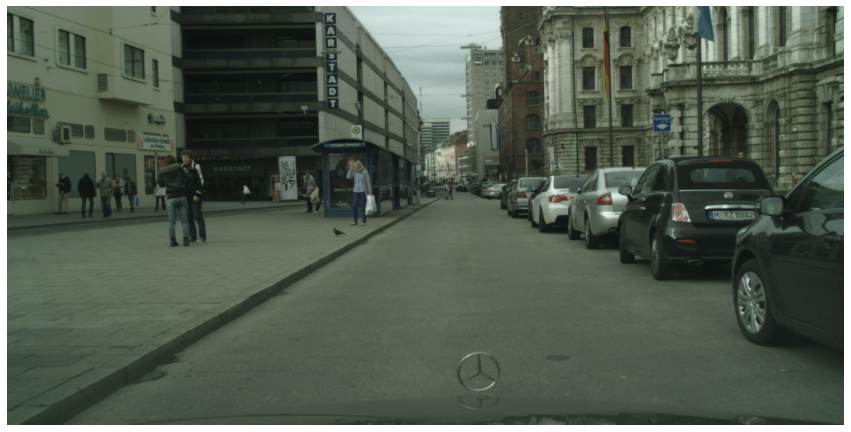
\includegraphics[width=.5\linewidth]{Obrazy/Rozdzial05/learning/3/r152l3.png}} 
        \subfloat[ResNet101.]{\label{101lr3}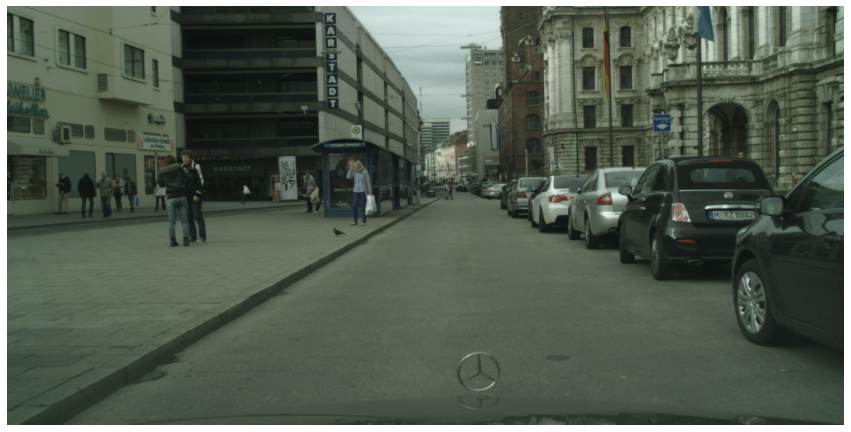
\includegraphics[width=.5\linewidth]{Obrazy/Rozdzial05/learning/3/r152l3.png}}\hfill
    \end{figure}
    \begin{figure}[H]\ContinuedFloat
    \centering
        \subfloat[ResNet152.]{\label{152lr3}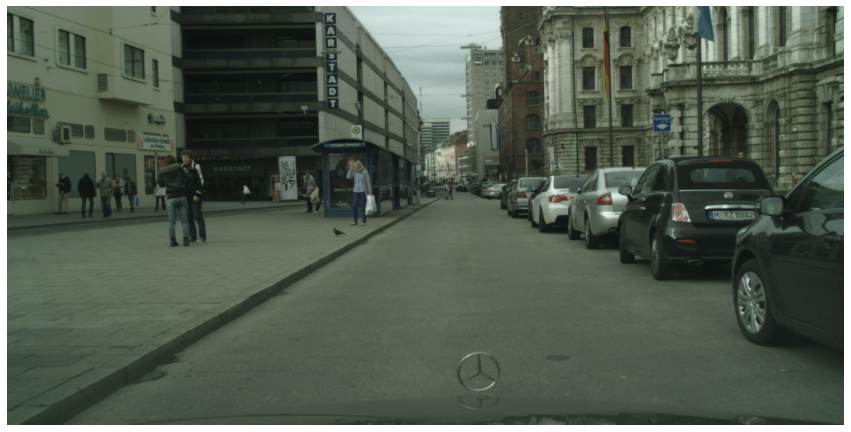
\includegraphics[width=.5\linewidth]{Obrazy/Rozdzial05/learning/3/r152l3.png}}
        \subfloat[VGG19.]{\label{19lr3}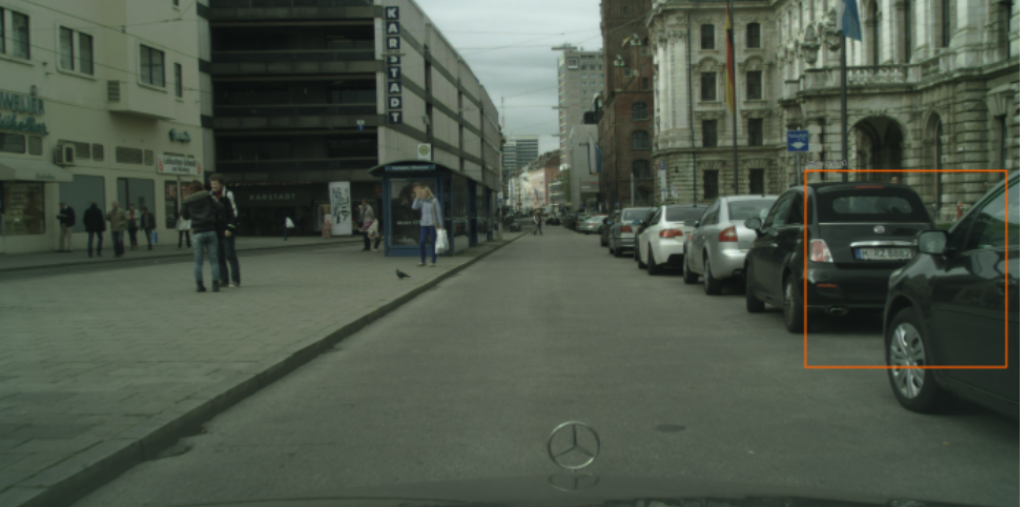
\includegraphics[width=.5\linewidth]{Obrazy/Rozdzial05/learning/3/19l3.png}}\hfill
    \caption{Porównanie wyników detekcji dla różnych architektur sieci dla \emph{lr} = $10^{-3}$.}
    \label{fig:lr_porównanie_3_zdj}
\end{figure}

\hspace{0.5cm}
We wszystkich przypadkach przedstawionych powyżej wartość szybkości uczenia okazała się zbyt duża, przez co sieć nie była w stanie się nic nauczyć lub wyniki były nieprecyzyjne i niepełne, jak w~przypadku modelu VGG19 pokazanego w \ref{19lr3}. Współczynnik uczenia wpływa na jego szybkość oddziałując bezpośrednio na gradient zmiany. W tym przypadku zbyt duża wartość sprawiła, że poruszał się on "dużymi krokami" pomijając zagłębienia z minimami. Wyniki przedstawione na zdjęciach odzwierciedlają również wartości metryki AP, gdzie w większości przypadków wynoszą 0 lub niewielkie wartości.

\begin{table}[H]
    \centering
    \caption{Zestawienie metryk AP dla modeli o parametrze \emph{lr}=$10^{-3}$.}
    \begin{tabular}{|c||c|c|c|c|}
    \hline
        \multirow{2}{*}{Architektura}&\multicolumn{3}{c|}{Metryka AP}\\ \cline{2-4}
         & 0.5:0.95&0.5&0.75\\ \hline \hline
        ResNet50 & 0.000 & 0.000 & 0.000 \\ \hline
        ResNet101 & 0.000 & 0.000 & 0.000 \\ \hline
        ResNet152 & 0.000 & 0.000 & 0.000 \\ \hline
        VGG19 & 0.004 & 0.016 & 0.001 \\ \hline
    \end{tabular}
    \label{tab:ap_lr3}
\end{table}

\hspace{0.5cm}
Kolejno przedstawione zostały wyniki dla parametru \emph{lr}=$10^{-5}$.

\begin{figure}[H]
    \centering
        \subfloat[ResNet50.]{\label{50lr5}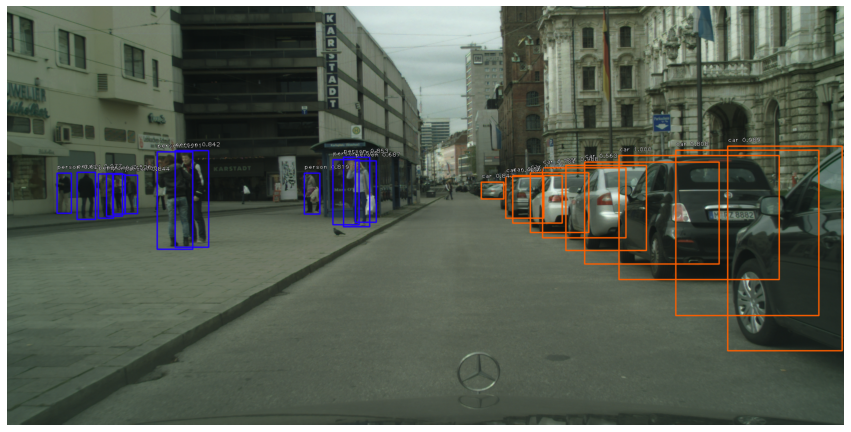
\includegraphics[width=.5\linewidth]{Obrazy/Rozdzial05/learning/5/r50l5.png}} 
        \subfloat[ResNet101.]{\label{101lr5}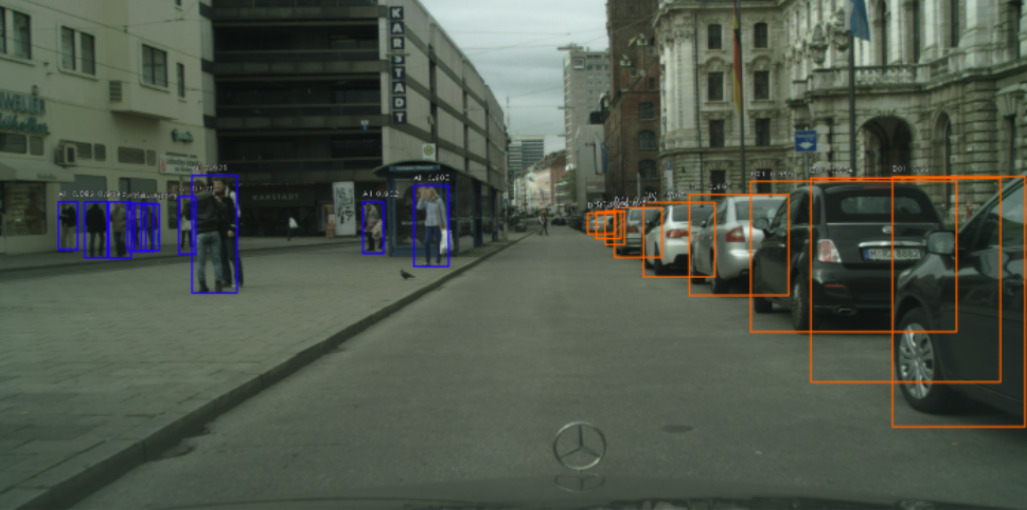
\includegraphics[width=.5\linewidth]{Obrazy/Rozdzial05/learning/5/r101l5.png}}\hfill
    \end{figure}
    \begin{figure}[H]\ContinuedFloat
    \centering
        \subfloat[ResNet152.]{\label{152lr5}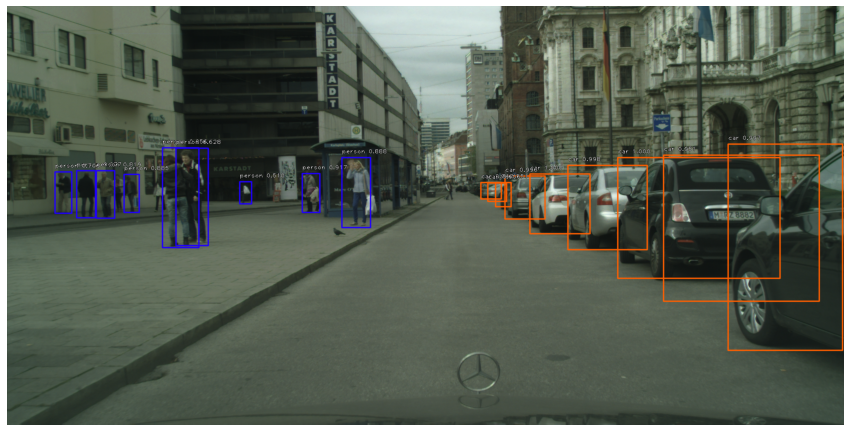
\includegraphics[width=.5\linewidth]{Obrazy/Rozdzial05/learning/5/r152l5.png}}
        \subfloat[VGG19.]{\label{19lr5}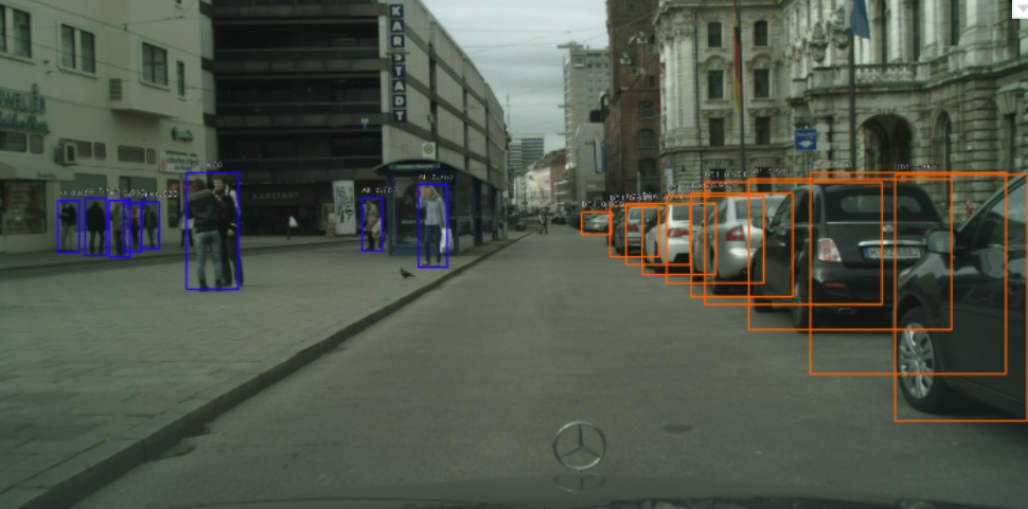
\includegraphics[width=.5\linewidth]{Obrazy/Rozdzial05/learning/5/19l5.png}}\hfill
    \caption{Porównanie wyników detekcji dla różnych architektur sieci dla \emph{lr} = $10^{-5}$.}
    \label{fig:lr_porównanie_5_zdj}
\end{figure}

\hspace{0.5cm}
Zastosowanie mniejszego współczynnika zdecydowanie poprawiło jakość modelu i wykonywanych detekcji. W niektórych przypadkach jednak występują fałszywie zakreślone obiekty, których tam nie ma lub wyniki są podwojone.
\begin{table}[H]
    \centering
        \caption{Zestawienie metryk AP dla modeli o parametrze \emph{lr}=$10^{-5}$.}
    \begin{tabular}{|c||c|c|c|c|}
    \hline
        \multirow{2}{*}{Architektura}&\multicolumn{3}{c|}{Metryka AP}\\ \cline{2-4}
         & 0.5:0.95&0.5&0.75\\ \hline \hline
        ResNet50 & 0.155 & 0.302 & 0.138 \\ \hline
        ResNet101 & 0.168 & 0.321 & 0.153 \\ \hline
        ResNet152 & 0.184 & 0.350 & 0.172 \\ \hline
        VGG19 & 0.122 & 0.242 & 0.105 \\ \hline
    \end{tabular}
    \label{tab:ap_lr5}
\end{table}

\hspace{0.5cm}
Ostatnia zastosowana wartość parametru wynosi \emph{lr}=$10^{-7}$.

\begin{figure}[H]
\centering
\subfloat[ResNet50.]{\label{50lr7}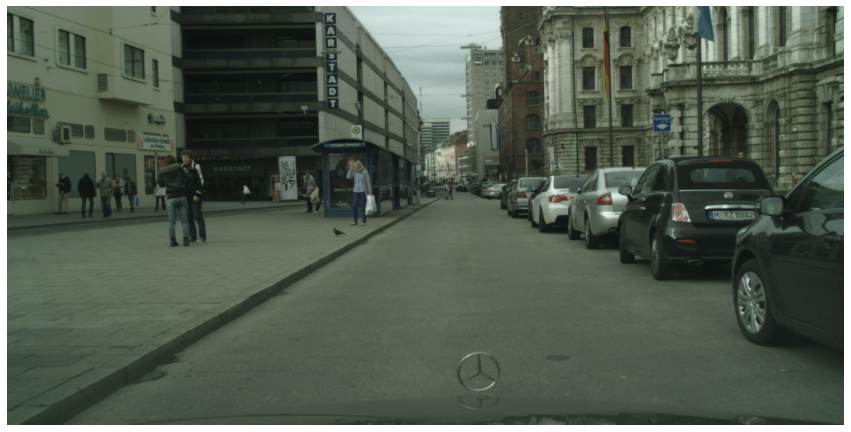
\includegraphics[width=.5\linewidth]{Obrazy/Rozdzial05/learning/7/r50l7.png}} 
\subfloat[ResNet101.]{\label{101lr7}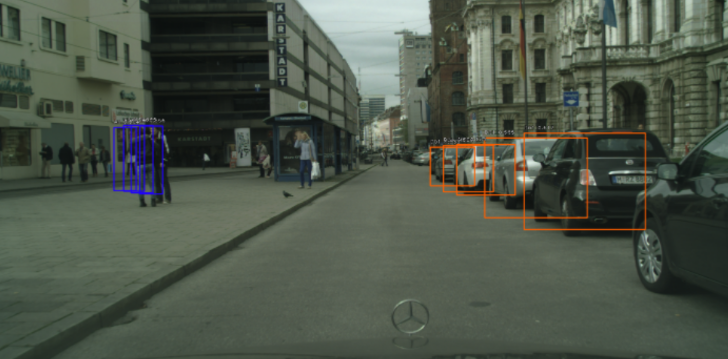
\includegraphics[width=.5\linewidth]{Obrazy/Rozdzial05/learning/7/r101l7.png}}\hfill
\end{figure}
\begin{figure}[H]\ContinuedFloat
\centering
\subfloat[ResNet152.]{\label{152lr7}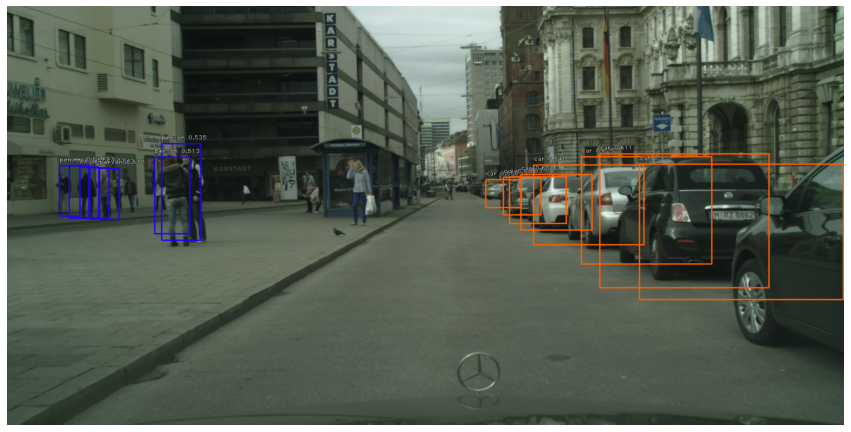
\includegraphics[width=.5\linewidth]{Obrazy/Rozdzial05/learning/7/r152l7.png}}
\subfloat[VGG19.]{\label{19lr7}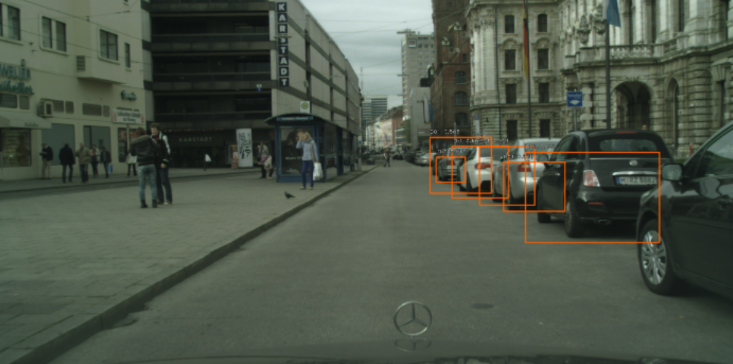
\includegraphics[width=.5\linewidth]{Obrazy/Rozdzial05/learning/7/19l7.png}}\hfill
\caption{Porównanie wyników detekcji dla różnych architektur sieci dla \emph{lr} = $10^{-7}$.}
\label{fig:lr_porównanie_7_zdj}
\end{figure}

\hspace{0.5cm}
W przeciwieństwie do pierwszego przypadku, zbyt mała wartość może spowodować, że podczas procesu sieć utknie w minimum lokalnym.
\begin{table}[H]
    \centering
    \caption{Zestawienie metryk AP dla modeli o parametrze \emph{lr}=$10^{-7}$.}
    \begin{tabular}{|c||c|c|c|c|}
    \hline
        &\multicolumn{3}{c|}{Metryka AP}\\ \cline{2-4}
        Architektura & 0.5:0.95&0.5&0.75\\ \hline \hline
        ResNet50 & 0.014 & 0.045 & 0.005 \\ \hline
        ResNet101 & 0.016 & 0.049 & 0.006 \\ \hline
        ResNet152 & 0.017 & 0.052 & 0.005 \\ \hline
        VGG19 & 0.007 & 0.0023 & 0.001 \\ \hline
    \end{tabular}
    \label{tab:ap_lr7}
\end{table}

\newpage
\hspace{0.5cm}
Wskazówką do wybrania odpowiedniego parametru \emph{lr} może być zbiór wykresów przedstawionych na rysunku \ref{fig:lr_teor}. Przedstawia on możliwe do otrzymania wykresy start, na których kształt wpływa wartość dobieranego parametru.

\begin{figure}[H]
    \centering
    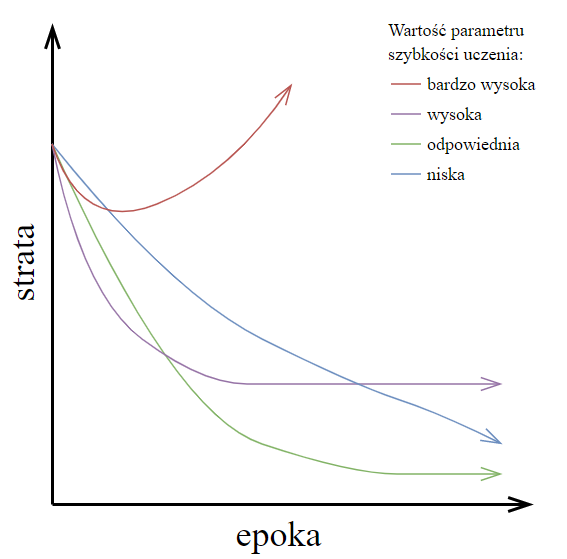
\includegraphics[width=0.5\linewidth]{Obrazy/Rozdzial05/learning/lr.png}
    \caption{Porównanie wykresów straty treningu w zależności od dobranej wartości parametru szybkości uczenia \emph{lr}.}
    \label{fig:lr_teor}
\end{figure}

\hspace{0.5cm}
W celu porównania wybrano jedną sieć, której wykresy dla każdego przypadku przedstawione poniżej porównano z przykładem \ref{fig:lr_teor}.
\begin{figure}[H]
\hspace{-2cm}
\subfloat[\emph{lr}=$10^{-3}$.]{\label{p3}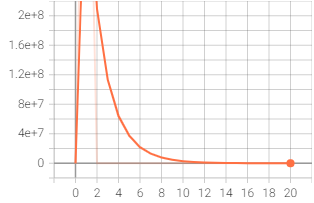
\includegraphics[width=.4\linewidth]{Obrazy/Rozdzial05/learning/ogol/l3.png}} 
\subfloat[\emph{lr}=$10^{-5}$.]{\label{p5}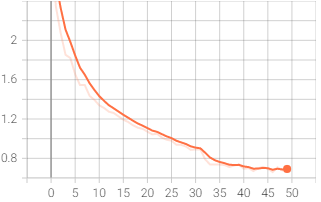
\includegraphics[width=.4\linewidth]{Obrazy/Rozdzial05/learning/ogol/l5.png}}
\subfloat[\emph{lr}=$10^{-7}$.]{\label{p3}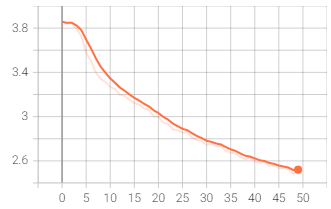
\includegraphics[width=.4\linewidth]{Obrazy/Rozdzial05/learning/ogol/l7.png}}\hfill
\caption{Porównanie wykresów strat dla modelu typu ResNet152.}
\label{fig:lr_porównanie_calk}
\end{figure}

\hspace{0.5cm}
Zgodnie z założeniem $10^{-3}$ jest zbyt duża do trenowania badanych sieci, a skok wartości na początku procesu uczenia sprawia, że wykres staje się nieczytelny. Mała wartość parametru \emph{lr} będzie znacznie wydłużać proces uczenia. Oznacza to, że o ile sieć mogła nie osiągnąć wystarczających wyników przy takiej samej ilości epok jak w pozostałych przypadkach, to po zwiększeniu ich ilości istnieje szansa poprawienia jakości modelu.

\newpage
\subsection{Wpływ wielkości partii}
\hspace{0.5cm}
W trakcie uczenia możliwa była zmiana ilości próbek (ang. \emph{batch size}), które zostaną jednocześnie przekazane do sieci.
Wygenerowane wykresy procesu uczenia dla każdego modelu zostały przedstawione na rysunku \ref{fig:batch_porównanie}, gdzie zmieniana była wartość wsadu danych przy identycznych pozostałych parametrach i zbiorze.

\begin{figure}[H]
\hspace{-1.5cm}
\subfloat[ResNet50, \emph{batch} = 1.]{\label{50b1}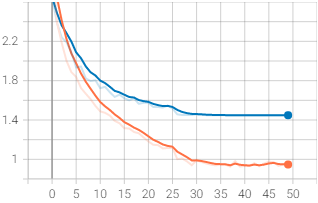
\includegraphics[width=.4\linewidth]{Obrazy/Rozdzial05/batch/RESNET50/B1/strata.png}}
\subfloat[ResNet50, \emph{batch} = 2.]{\label{50b2}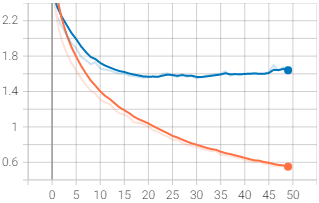
\includegraphics[width=.4\linewidth]{Obrazy/Rozdzial05/batch/RESNET50/B2/strata.png}}
\subfloat[ResNet50, \emph{batch} = 3.]{\label{50b3}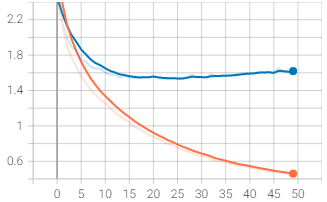
\includegraphics[width=.4\linewidth]{Obrazy/Rozdzial05/batch/RESNET50/B3/strata.png}}\hfill
\end{figure}
\begin{figure}[H]\ContinuedFloat
\hspace{-1.5cm}
\subfloat[ResNet101, \emph{batch} = 1.]{\label{101b1}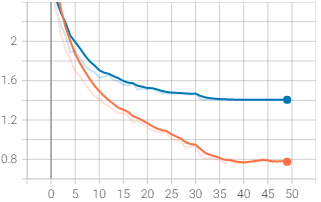
\includegraphics[width=.4\linewidth]{Obrazy/Rozdzial05/batch/RESNET101/B1/strata.png}}
\subfloat[ResNet101, \emph{batch} = 2.]{\label{101b2}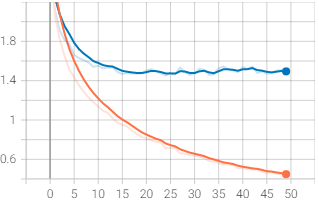
\includegraphics[width=.4\linewidth]{Obrazy/Rozdzial05/batch/RESNET101/B2/strata.png}}
\subfloat[ResNet101, \emph{batch} = 3.]{\label{101b3}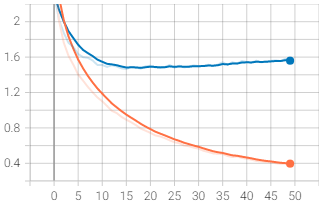
\includegraphics[width=.4\linewidth]{Obrazy/Rozdzial05/batch/RESNET101/B3/strata.png}}\hfill
\end{figure}
\begin{figure}[H]\ContinuedFloat
\hspace{-1.5cm}
\subfloat[ResNet152, \emph{batch} = 1.]{\label{152b1}\includegraphics[width=.4\linewidth]{Obrazy/Rozdzial05/batch/RESNET152/B1/strata.png}}
\subfloat[ResNet152, \emph{batch} = 2.]{\label{152b2}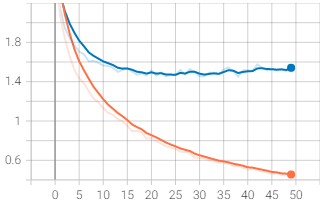
\includegraphics[width=.4\linewidth]{Obrazy/Rozdzial05/batch/RESNET152/B2/strata.png}}
\subfloat[ResNet152, \emph{batch} = 3.]{\label{152b3}\includegraphics[width=.4\linewidth]{Obrazy/Rozdzial05/batch/RESNET152/B3/strata.png}}\hfill
\end{figure}
\begin{figure}[H]\ContinuedFloat
\hspace{-1.5cm}
\subfloat[VGG19, \emph{batch} = 1.]{\label{19b1}\includegraphics[width=.4\linewidth]{Obrazy/Rozdzial05/batch/VGG19/B1/strata.png}}
\subfloat[\VGG19, \emph{batch} = 2.]{\label{19b2}\includegraphics[width=.4\linewidth]{Obrazy/Rozdzial05/batch/VGG19/B1/strata.png}}
\subfloat[VGG19, \emph{batch} = 3.]{\label{19b3}\includegraphics[width=.4\linewidth]{Obrazy/Rozdzial05/batch/VGG19/B3/strata.png}}\hfill
\caption{Porównanie wykresów straty treningu i walidacji dla różnych architektur sieci w zależności od zastosowanej wielkości wsadu danych\emph{batch}.}
\label{fig:batch_porównanie}
\end{figure}


% Teoretycznie szybsze 
% Po pierwsze, generalnie im większy rozmiar partii, tym szybciej nasz model ukończy każdą epokę podczas treningu. Dzieje się tak, ponieważ w zależności od naszych zasobów obliczeniowych nasza maszyna może przetwarzać znacznie więcej niż jedną próbkę na raz.

% Kompromis polega jednak na tym, że nawet jeśli nasza maszyna może obsługiwać bardzo duże partie, jakość modelu może się pogorszyć, gdy ustawimy większą partię, co może ostatecznie spowodować, że model nie będzie w stanie dobrze uogólnić danych, których nie miał widział.

\hspace{0.5cm}
Wykorzystanie jednocześnie większej ilości danych w jednej iteracji zwiększa zapotrzebowanie na pamięć, przez co nie każda maszyna jest w stanie obsługiwać bardzo duże partie danych jednocześnie. Wielkość partii może również negatywnie wpłynąć na sam model. Wraz ze wzrostem wielkości wsadu zdjęć model szybciej osiąga swoją minimalną wartość błędu walidacji (przykłady \ref{50b3}, \ref{101b3}, \ref{152b3} i \ref{19b3}), jednak w przeciwieństwie do wsadu równego 1 nie stabilizuje się, natomiast zaczyna rosnąć, co oznacza przeuczenie modelu i dyskwalifikuje go z~użytkowania w praktyce.

\begin{figure}[H]
\hspace{-1.5cm}
\subfloat[Detekcja obiektów z wykorzystaniem modelu \\ ResNet50, \emph{batch} = 1.]{\label{bp1}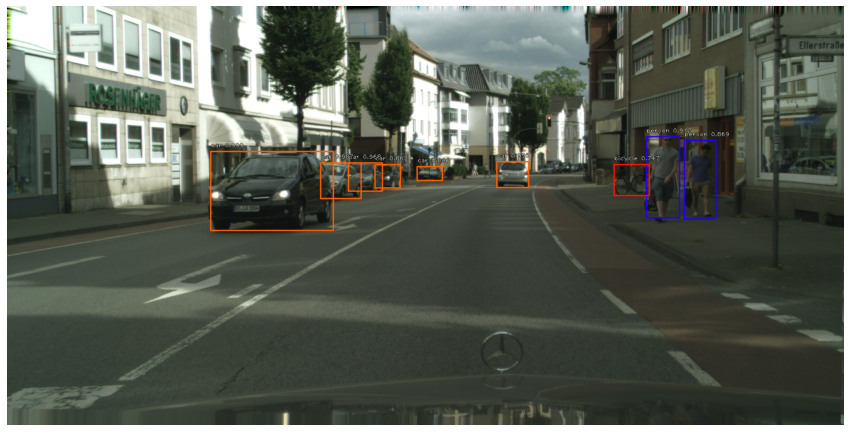
\includegraphics[width=.6\linewidth]{Obrazy/Rozdzial05/batch/RESNET50/zdjecia/res50b1.png}}
\subfloat[Detekcja obiektów z wykorzystaniem modelu \\ ResNet50, \emph{batch} = 3.]{\label{bp2}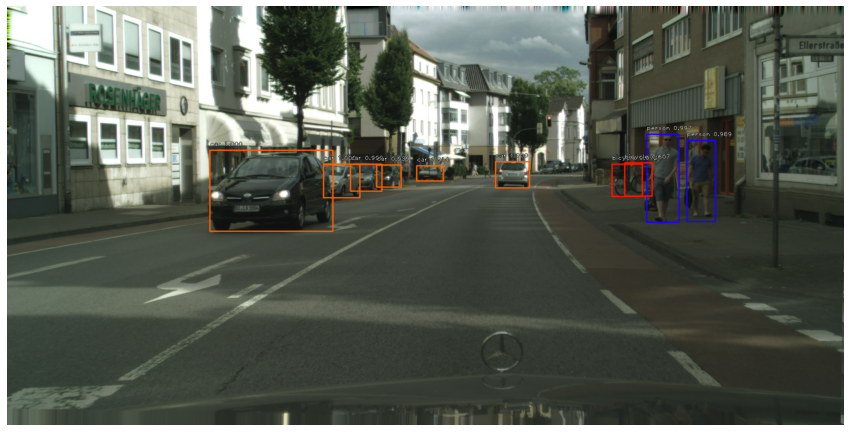
\includegraphics[width=.6\linewidth]{Obrazy/Rozdzial05/batch/RESNET50/zdjecia/res50b3.png}}\hfill
\end{figure}
\begin{figure}[H]\ContinuedFloat
\hspace{-1.5cm}
\subfloat[Detekcja obiektów z wykorzystaniem modelu \\ VGG19, \emph{batch} = 1.]{\label{bp3}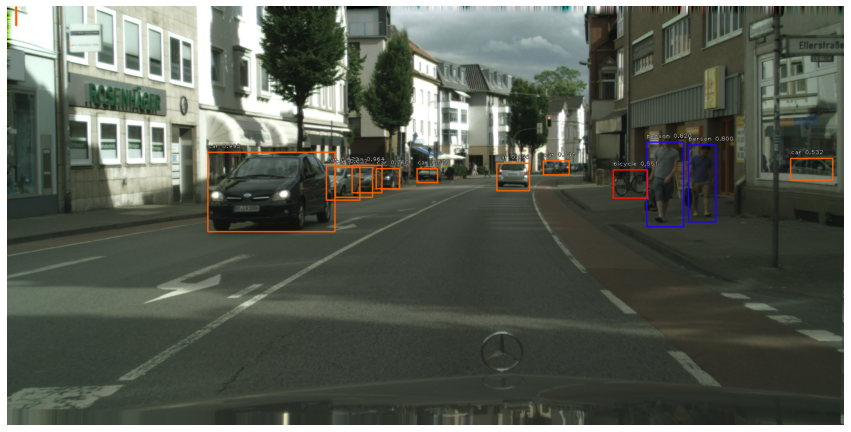
\includegraphics[width=.6\linewidth]{Obrazy/Rozdzial05/batch/VGG19/zdjecia/vgg19b1.png}}
\subfloat[Detekcja obiektów z wykorzystaniem modelu \\ VGG19, \emph{batch} = 3.]{\label{bp4}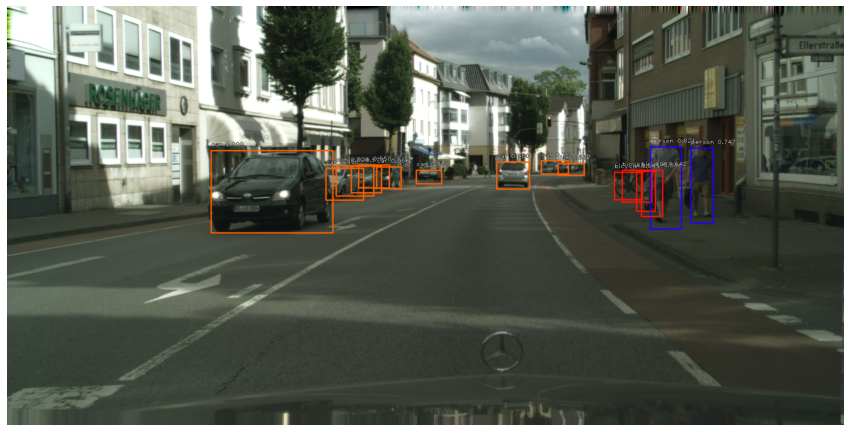
\includegraphics[width=.6\linewidth]{Obrazy/Rozdzial05/batch/VGG19/zdjecia/vgg19b3.png}}\hfill
\caption{Porównanie obiektów wykrytych na zdjęciach.}
\label{fig:batch_zdjecia}
\end{figure}

\hspace{0.5cm}
Porównując wyniki ze zdjęć \ref{fig:batch_porównanie} i \ref{fig:batch_zdjecia} widoczne jest, że mimo podobnych wyników detekcji, model trenowany na danych podawanych w większych zbiorach wykazuje skłonności do poprawnych, ale podwójnych detekcji.

\subsection{Wybór najlepszego modelu}
\label{najlepszy}

\hspace{0.5cm}
Po przeanalizowaniu wyżej wymienionych wyników uczenia wszystkie sieci douczono lub stworzono nowe modele z ponownie dobranymi parametrami tj. zwiększona ilość epok, wybranie istotnych wartości parametry \emph{lr}, dobranie odpowiedniej wielkości parametru \emph{batch} oraz zwiększenie ilości zdjęć. Spośród nich wybrano model, którego błędy straty i walidacji nie ustabilizowany się przy zakończeniu uczenia ani nie wskazywały na jego przeuczenie w celu douczenia go do uzyskania satysfakcjonujących wartości.

\begin{figure}[H]
\centering
\subfloat[Wykres strat treningu i walidacji \\ modelu  przed douczeniem.]{\label{d1}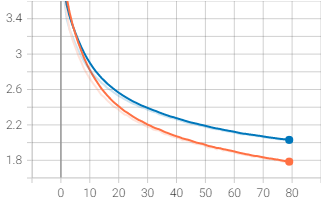
\includegraphics[width=.4\linewidth]{Obrazy/Rozdzial05/najlepszymodel/stratap.png}}
\subfloat[Wykres strat treningu i walidacji modelu po douczeniu.]{\label{d2}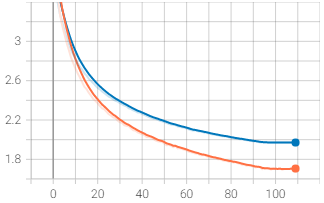
\includegraphics[width=.4\linewidth]{Obrazy/Rozdzial05/najlepszymodel/strata.png}}\hfill
\subfloat[Wykres wartości parametru szybko-\\ści uczenia przed douczeniem.]{\label{d3}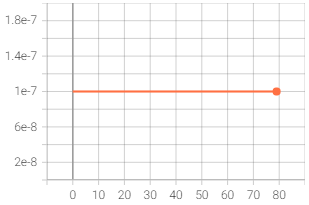
\includegraphics[width=.4\linewidth]{Obrazy/Rozdzial05/najlepszymodel/lrp.png}}
\subfloat[Wykres wartości parametru szybkości uczenia po douczeniu.]{\label{d4}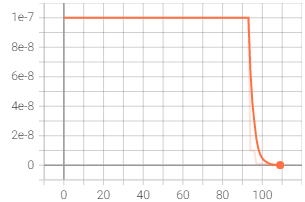
\includegraphics[width=.4\linewidth]{Obrazy/Rozdzial05/najlepszymodel/lr.png}}\hfill
\caption{Informacje związane z modelem wybranym do dalszego uczenia.}
\label{fig:dotrenowany}
\end{figure}

\hspace{0.5cm}
Tak dotrenowany model porównany został z modelem wytrenowanym i udostępnionym do użytku powszechnego \cite{best}.

\begin{figure}[H]
\hspace{-1.5cm}
\subfloat[Detekcja obiektów douczonym modelem.]{\label{d1}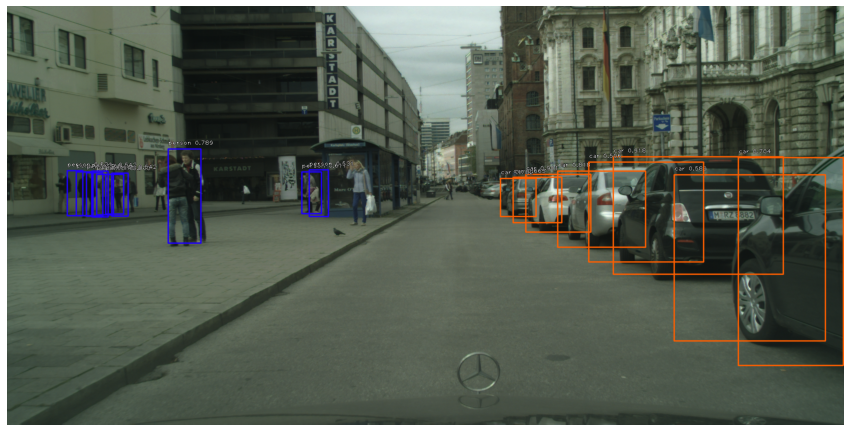
\includegraphics[width=.6\linewidth]{Obrazy/Rozdzial05/najlepszymodel/zdjN.png}}
\subfloat[Detekcja obiektów gotowym modelem.]{\label{w1}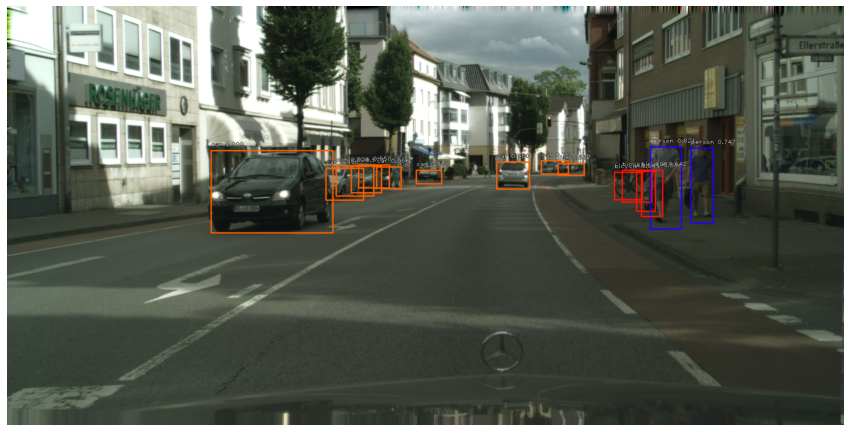
\includegraphics[width=.6\linewidth]{Obrazy/Rozdzial05/batch/VGG19/zdjecia/vgg19b3.png}}\hfill
\end{figure}
\begin{figure}[H]\ContinuedFloat
\hspace{-1.5cm}
\subfloat[Detekcja obiektów douczonym modelem.]{\label{d2}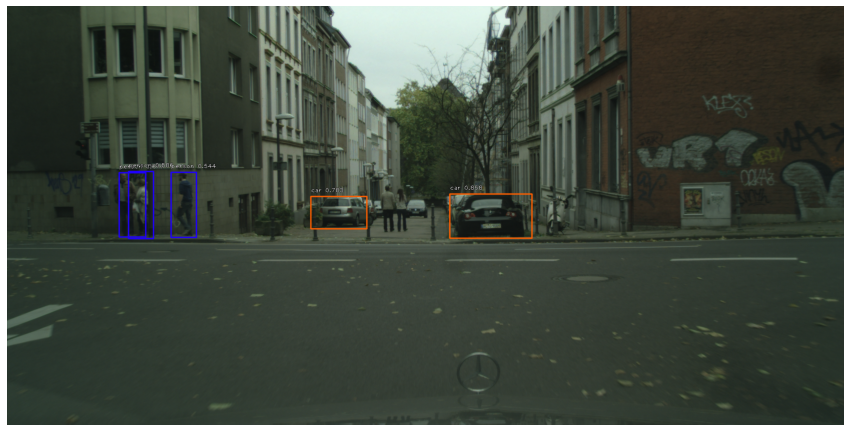
\includegraphics[width=.6\linewidth]{Obrazy/Rozdzial05/najlepszymodel/zdjN3.png}}
\subfloat[Detekcja obiekt gotowym modelem.]{\label{w2}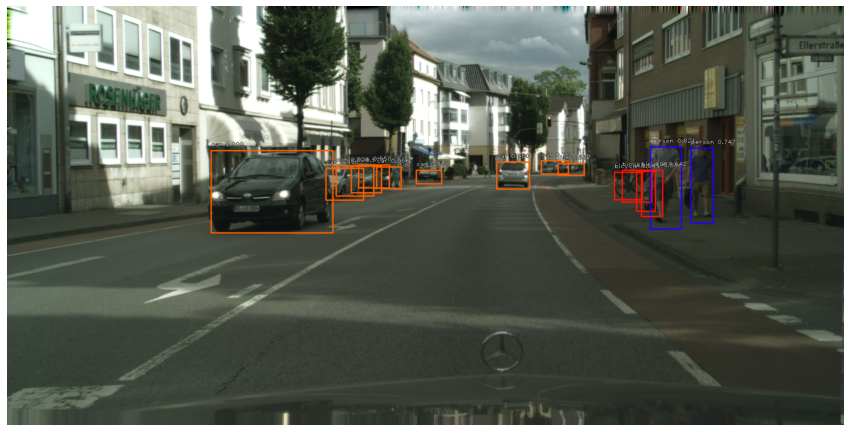
\includegraphics[width=.6\linewidth]{Obrazy/Rozdzial05/batch/VGG19/zdjecia/vgg19b3.png}}\hfill
\caption{Porównanie obiektów wykrytych na zdjęciach.}
\label{fig:p_wd}
\end{figure}



\section{Detekcja sytuacji niebezpiecznych}
\hspace{0.5cm}
Korzystając z repozytorium Fizyr oraz wybranych modeli sieci, utworzony został program służący do analizy obrazu pod kątem wykrywania niebezpiecznych sytuacji na drodze. Składa się on z plików zawierających

\begin{itemize}
    \item[--] detect.py - funkcje odpowiadające za przyjęcie parametrów tj. rodzaju architektury i wybranego modelu, typu wprowadzanych mediów oraz ścieżka do pliku wideo/zdjęcia lub kamery, z której czerpany ma być obraz,

    \begin{code}
    \captionof{listing}{Funkcja służąca do wczytywania wprowadzanych paramaterów.}
    \label{code:c-code}
    \begin{minted}[Python, linenos,tabsize=2,breaklines, framesep=2mm]{Python}
    def parse_args(args):
        parser = argparse.ArgumentParser(description='Program do wykrywania zagrożeń na drodze.')
        
        group = parser.add_mutually_exclusive_group()
        parser.add_argument('--backbone',    help='Backbone model used by retinanet.',       
        default='ResNet50', type=str)
        parser.add_argument('--model-dir',   help='Path to model.', default='', type=str) 
        parser.add_argument('--media',       help='Media type.', default='photo', type=str) 
        parser.add_argument('--media-dir',   help='Media type.', default='', type=str) 
        
        return check_args(parser.parse_args(args))
    \end{minted}
    \end{code}

    \item[--] utility.py - zbiór funkcji służących do przetwarzania obrazów i graficznego przedstawienia wykrytych sytuacji, wykorzystywanych następnie przez odpowiednie klasy w zależności od rodzaju podanych mediów przez odpowiednie klasy,
    \item[--] detect\_dangerous.py - klasę określającą przestrzeń przed maską samochodu i status badanej sytuacji (bezpieczna/niebezpieczna),
    \item[--] detect\_photo.py - klasę przetwarzającą zdjęcie podane przez użytkownika, zakreślającą obszar na jakim znajduje się wykryty obiekt, generującą końcowy obraz,
    \item[--] detect\_movies.py - klasę przetwarzającą kolejno klatki filmu video lub kamery podane przez użytkownika, zakreślającą obszar na jakim znajduje się wykryty obiekt, generującą końcowy obraz w formie sekwencji zmieniających się klatek,
    
\end{itemize}

\hspace{0.5cm}
Jako sytuację niebezpieczną określono wszystkie zdarzenia prowadzące do znalezienia się przed pojazdem niespodziewanego obiektu tj. pieszy lub samochód przed. W celu określenia niebezpiecznego obszaru zakreślone zostało pole znajdujące się przed maską pojazdu, którym hipotetycznie porusza się użytkownik.

\begin{figure}[H]
    \centering
    \includegraphics[width=0.7\linewidth]{Obrazy/Rozdzial05/trapez.png}
    \caption{Sposób określenia pola przed samochodem.}
    \label{fig:trapez}
\end{figure}

\hspace{0.5cm}
Trapez został zdefiniowany, jako pewne punkty w pliku \emph{detect\_dangerous.py} możliwe do wprowadzenia przez użytkownika i uzależnione od rozdzielczości zdjęcia.

\begin{code}
    \captionof{listing}{Funkcja określająca sposób doboru punktów kształtu przed maską oraz wyznaczenia boków tego obszaru.}
    \label{code:c-code}
    \begin{minted}[Python, linenos,tabsize=2,breaklines, framesep=2mm]{Python}
    def __init__(self, media):
        if media == 'photo':
            self.start_right = (1330,600)
            self.end_right = (1900,1024)
            self.start_left = (850,600)
            self.end_left = (290,1024)
            self.top = 600
        
        if media == 'movie':
            self.start_right = (1150,720)
            self.end_right = (1780,1080)
            self.start_left = (910,720)
            self.end_left = (460,1080)
            self.top = 720

        self.wsp_a_r = (self.start_right[1]-self.end_right[1])/(self.start_right[0] -self.end_right[0])
        self.wsp_b_r = self.start_right[1] - self.wsp_a_r * self.start_right[0]

        self.wsp_a_l = (self.start_left[1]-self.end_left[1])/(self.start_left[0] -self.end_left[0])
        self.wsp_b_l = self.start_left[1] - self.wsp_a_l * self.start_left[0]
    \end{minted}
    \end{code}

\hspace{0.5cm}
 W trakcie działania programu sprawdzane są kolejno warunki, czy przynajmniej dwie z~krawędzi prostokątów otaczających wykryte obiekty częściowo znajdują się w zakresie trapezu rysowanego przed pojazdem. Wykonanie analizy możliwe było dla statycznie podanych zdjęć lub z sekwencji klatek filmowych np. z kamery samochodowej przedstawionej w~punkcie \ref{r:sanok}. Ze względu na dużą ilość informacji, które wymagają przetworzenia w krótkim czasie, do ewaluacji wybrana została co szósta klatka.
 
\hspace{0.5cm}
Jeżeli obiekt będący w polu widzenia pojazdu znajduje się na poboczu lub w odpowiedniej odległości przed maską samochodu, zostanie oznaczony zielonym obramowaniem. Jeżeli jednak jego położenie będzie nachodzić się z wyznaczonym obszarem przed maską, to zostanie on oznaczony czerwoną ramką w każdym momencie występowania. Sama ewaluacja wyników odbyła się na subiektywnej ocenie sytuacji na obrazie przez użytkownika.

\subsection{Piesi i samochody}
\hspace{0.5cm}
 Poniżej zestawione zostały różne sytuacje pochodzące ze zbioru, który nie brał udziału w~procesie uczenia sieci. Na zdjęciach \ref{fig:zdj_pop} przedstawiają poprawnie określone sytuacje niebezpieczne tj. odpowiednie określenie pieszych na przejściu, samochodów przez pojazdem. 

\begin{figure}[H]
\hspace{2.4cm}
\subfloat[Prawidłowo oznaczone obiekty w bezpiecznej sytuacji.]{\label{z1p}\includegraphics[width=.7\linewidth]{Obrazy/Rozdzial05/program/resnet152/poprawne/best_pic1.png}}\hfill
\end{figure}
\begin{figure}[H]\ContinuedFloat
\centering
\subfloat[Prawidłowo oznaczone obiekty w bezpiecznej sytuacji.]{\label{z2p}\includegraphics[width=.7\linewidth]{Obrazy/Rozdzial05/program/resnet152/poprawne/best_pic11.png}}\hfill
\subfloat[Prawidłowo oznaczone obiekty w niebezpiecznej sytuacji.]{\label{z3p}\includegraphics[width=.7\linewidth]{Obrazy/Rozdzial05/program/resnet152/poprawne/best_pic31.png}}\hfill
\subfloat[Prawidłowo oznaczone obiekty w niebezpiecznej sytuacji.]{\label{z4p}\includegraphics[width=.7\linewidth]{Obrazy/Rozdzial05/program/resnet152/poprawne/best_pic18.png}}\hfill
\caption{Poprawnie przeanalizowane klatki materiału wideo kamery samochodowej.}
\label{fig:zdj_pop}
\end{figure}

\hspace{0.5cm}
Wykorzystywany model nie przedstawia kompletnych wyników np. brak osób na chodniku \ref{z3p} i \ref{z4p}, jednak główne elementy mogące znaleźć się przed pojazdem zostają odpowiednio zaznaczone.

\hspace{0.5cm}
Pomimo częściowo zadowalających wyników w czasie detekcji można było napotkać błędy wynikające z działania modelu lub zakresu określonego przed pojazdem.

\begin{figure}[H]
\centering
\subfloat[Nieprawidłowo oznaczone obiekty w niebezpiecznej sytuacji.]{\label{z1n}\includegraphics[width=.7\linewidth]{Obrazy/Rozdzial05/program/resnet152/niepoprawne/best_pic29.png}}\hfill
\subfloat[Nieprawidłowo oznaczone obiekty w bezpiecznej sytuacji.]{\label{z2n}\includegraphics[width=.7\linewidth]{Obrazy/Rozdzial05/program/resnet152/niepoprawne/best_pic66.png}}\hfill
\subfloat[Nieprawidłowo oznaczone obiekty w bezpiecznej sytuacji.]{\label{z3n}\includegraphics[width=.7\linewidth]{Obrazy/Rozdzial05/program/resnet152/niepoprawne/best_pic73.png}}
\end{figure}
\begin{figure}[H]\ContinuedFloat
\centering
\subfloat[Nieprawidłowo oznaczone obiekty w bezpiecznej sytuacji.]{\label{z4n}\includegraphics[width=.7\linewidth]{Obrazy/Rozdzial05/program/resnet152/niepoprawne/coco_pic30.png}}\hfill
\caption{Przeanalizowane klatki materiału wideo kamery samochodowej zawierające błędy.}
\label{fig:zdj_niepop}
\end{figure}

\hspace{0.5cm}
Główne problemy wynikały z niewystarczającego wyuczenia modelu, który nie zawsze był w stanie wykryć obiekty, które znajdowały się w badanej sytuacji (\ref{z1n}). Innym powodem błędnych oznaczeń niebezpieczeństwa jest nieodpowiednio zakreślony obszar detekcji przed samochodem. Zbyt krótki nie informuje użytkownika w porę o zbliżającym się możliwym niebezpieczeństwie, natomiast zbyt długi może doprowadzić do alarmowego oznaczenia obiektów nie znajdujących się na drodze kolizyjnej z pojazdem (\ref{z3n} i \ref{z4n}).

\subsection{Porównanie z gotowym modelem}

\hspace{0.5cm}
Do analizy tego samego materiału wideo wykorzystano również gotowy model przedstawione w punkcie \ref{najlepszy} w celu porównania wybranych wyników detekcji.

\begin{figure}[H]
\hspace{2.4cm}
\subfloat[Detekcja wykonana douczonym modelem.]{\label{dd1}\includegraphics[width=.7\linewidth]{Obrazy/Rozdzial05/program/resnet152/niepoprawne/best_pic26.png}}\hfill
\end{figure}
\begin{figure}[H]\ContinuedFloat
\centering
\subfloat[Detekcja wykonana gotowym modelem.]{\label{dd2}\includegraphics[width=.7\linewidth]{Obrazy/Rozdzial05/program/resnet50/poprawne/coco_pic26.png}}\hfill
\subfloat[Detekcja wykonana douczonym modelem.]{\label{dd1}\includegraphics[width=.7\linewidth]{Obrazy/Rozdzial05/program/resnet152/niepoprawne/best_pic66.png}}\hfill
\subfloat[Detekcja wykonana gotowym modelem.]{\label{dd2}\includegraphics[width=.7\linewidth]{Obrazy/Rozdzial05/program/resnet50/poprawne/coco_pic66.png}}\hfill
\caption{Porównanie identycznych sytuacji wykorzystując dwa wybrane modele.}
\label{fig:model_por}
\end{figure}


\subsection{Ubytki w nawierzchni}
\hspace{0.5cm}
W celu detekcji uszkodzeń nawierzchni uczony został osobny model o parametrach wybranych w punkcie \ref{najlepszy}. Spowodowane było to różnicami pomiędzy formatem wykorzystywanego zbioru zdjęć, gdzie drogi przedstawione zostały w~formacje Pascal VOC oraz różniącymi klasami w plikach adnotacji. Poniżej zostały przedstawione wybrane wyniki detekcji uszkodzeń dla jednego z wytrenowanych modeli.

\begin{figure}[H]
\centering
\subfloat[Prawidłowo wykryty i oznaczony obiekt.]{\label{w1}\includegraphics[width=.45\linewidth]{Obrazy/Rozdzial05/program/dziury/pic50_1.png}}
\subfloat[Prawidłowo wykryty i oznaczony obiekt.]{\label{w2}\includegraphics[width=.45\linewidth]{Obrazy/Rozdzial05/program/dziury/pic50_2.png}}\hfill
\subfloat[Niepełna detekcja obiektów na zdjęciu.]{\label{w3}\includegraphics[width=.45\linewidth]{Obrazy/Rozdzial05/program/dziury/pic50_3.png}}
\subfloat[Nieprawidłowa analiza zdjęcia.]{\label{w4}\includegraphics[width=.45\linewidth]{Obrazy/Rozdzial05/program/dziury/pic50_4.png}}\hfill
\caption{Wyniki analizy obrazu trenowanym modelem sieci.}
\label{fig:dziura}
\end{figure}

\section{Omówienie wyników}